\chapter*{Conclusion}
\addcontentsline{toc}{chapter}{Conclusion} % Adding toc entry


\section*{Synthèse du travail accompli}

La digitalisation croissante des services de mobilité a rendu la qualité et la cohérence des données de transport public plus cruciales que jamais. Ce projet est né du constat d'un \textbf{désalignement} persistant entre la base de données officielle des arrêts en Suisse, ATLAS, et la référence cartographique collaborative mondiale, OpenStreetMap (OSM). Ces divergences, qu'elles soient de nature géographique, nominative ou structurelle, engendrent des incohérences qui dégradent l'expérience des usagers et complexifient les opérations pour les planificateurs.

Après filtrage, \textbf{54\,880} arrêts ATLAS (\texttt{BOARDING\_PLATFORM}) ont été retenus. 
Pour répondre à cette problématique, nous avons conçu et mis en œuvre une solution complète en trois phases. La première phase a consisté à développer un \textbf{pipeline de traitement automatisé} en Python, appliquant une cascade de méthodes d'appariement : correspondance exacte par identifiants, par nom, par proximité géographique, et enfin par analyse des lignes de transport (GTFS et HRDF). 

Les résultats quantitatifs sont significatifs : nous avons réussi à établir \textbf{48\,213} correspondances, ce qui représente une couverture de \textbf{85,0\%} des arrêts ATLAS distincts (\(46\,611/54\,880\)). Ce processus a également permis de cataloguer et de prioriser des milliers d'anomalies, incluant \textbf{11\,126} problèmes de distance, \textbf{27\,376} non-appariements et \textbf{15\,963} conflits d'attributs (voir Chapitre~6). Les tableaux suivants détaillent (i) la répartition des correspondances par méthode et (ii) les problèmes de \textbf{priorité maximale (P1)}.

\vspace{0.5em}
\section*{Correspondances par méthode}
\begin{table}[h]
\centering
\caption{Correspondances par méthode (sur \textbf{48\,213} correspondances)}
\label{tab:matches_by_method_conclusion}
\begin{tabular}{|l|r|r|}
\hline
\textbf{Méthode} & \textbf{Nombre} & \textbf{Part (\%)} \\
\hline
Correspondances exactes & 21\,124 & 43,8 \\
Correspondances par nom & 535 & 1,1 \\
Correspondances par distance & 18\,661 & 38,7 \\
Correspondances par routes & 6\,944 & 14,4 \\
Consolidation post-traitement & 883 & 1,8 \\
Propagation des duplicatas & 66 & 0,1 \\
\hline
\textbf{Total} & \textbf{48\,213} & \textbf{100,0} \\
\hline
\end{tabular}
\end{table}

\noindent\small Détail des correspondances par distance: Étape\,1 (groupe–proximité)\,=\,15\,384; Étape\,2 (référence locale)\,=\,129; Étape\,3a (candidat unique)\,=\,2\,012; Étape\,3b (ratio de distance)\,=\,1\,136.

\noindent\small Précision: le \emph{Total de correspondances} correspond au nombre de paires ATLAS--OSM (\textbf{48\,213}), tandis que le \emph{Total d'arrêts avec correspondances} correspond au nombre d'arrêts ATLAS distincts appariés (\textbf{46\,611}), soit \textbf{85,0\%} des \textbf{54\,880} arrêts considérés.

\vspace{0.5em}
\section*{Problèmes de priorité maximale (P1)}
\begin{table}[h]
\centering
\caption{Problèmes de priorité P1 par type}
\label{tab:p1_problems_conclusion}
\begin{tabular}{|l|r|}
\hline
\textbf{Type de problème} & \textbf{P1 (nombre)} \\
\hline
Distance & 1\,277 \\
Non-appariements & 4\,903 \\
Attributs & 7\,387 \\
\hline
\textbf{Total P1} & \textbf{13\,567} \\
\hline
\end{tabular}
\end{table}

La deuxième phase a porté sur le développement d'une \textbf{application web full-stack} (Flask, SQLAlchemy, JavaScript) pour la validation humaine. Cette plateforme offre une interface cartographique interactive pour visualiser les données, un outil dédié pour trier et résoudre les problèmes détectés, et un mécanisme de \textbf{persistance des solutions}, assurant que les corrections manuelles sont conservées et réappliquées lors des futurs imports de données.

Enfin, la troisième phase a consisté à \textbf{sécuriser et conteneuriser} l'application. Nous avons implémenté un système d'authentification robuste (mots de passe hachés avec Argon2, authentification à deux facteurs, protection CSRF, limitation de débit) et déployé l'ensemble de la pile logicielle (backend, base de données MySQL, frontend) avec Docker, garantissant un déploiement reproductible et simplifié.

Au moment du dépôt, voici un résumé concis des principaux types de fichiers du dépôt, incluant les données, le pipeline d'appariement, l'application web et les scripts utilisés pour le rapport.

\begin{table}[h]
\centering
\caption{Résumé des lignes de code par type de fichier}
\label{tab:code_summary}
\begin{tabular}{|l|r|r|r|r|r|}
\hline
\textbf{Type de fichier} & \textbf{Fichiers} & \textbf{Total} & \textbf{Non vides} & \textbf{Commentaires} & \textbf{Code} \\
\hline
Python & 70 & 15\,006 & 12\,755 & 3\,051 & 9\,705 \\
HTML & 23 & 1\,667 & 1\,551 & 73 & 1\,478 \\
JavaScript & 17 & 7\,519 & 6\,706 & 771 & 5\,935 \\
CSS & 35 & 1\,681 & 1\,428 & 89 & 1\,339 \\
\hline
\textbf{TOTAL} & \textbf{145} & \textbf{25\,873} & \textbf{22\,440} & \textbf{3\,984} & \textbf{18\,457} \\
\hline
\end{tabular}
\end{table}

Le code Python, représentant \textbf{9\,705 lignes} réparties sur 70 fichiers, constitue l'épine dorsale du projet. Comme illustré dans la figure \ref{fig:python_distribution}, ce code présente deux aspects complémentaires : d'une part la \textbf{répartition du nombre de fichiers} par catégorie (visualisation de gauche), et d'autre part la \textbf{distribution des lignes de code} par catégorie (visualisation de droite).

Cette double perspective révèle des insights intéressants : alors que certaines catégories contiennent de nombreux fichiers relativement courts (comme les scripts du mémoire avec 24 fichiers), d'autres concentrent beaucoup de code dans peu de fichiers (comme les blueprints Flask avec seulement 6 fichiers mais 2\,173 lignes de code).

Le code se répartit principalement en trois catégories majeures :

\begin{itemize}
\item \textbf{Scripts du mémoire (26,1\% - 2\,534 lignes)} : scripts d'analyse et de visualisation utilisés pour la rédaction de ce rapport, incluant les statistiques d'appariement, les analyses de distribution de distance et la détection de problèmes.

\item \textbf{Backend de l'application web (29,4\% du total)} : 
\begin{itemize}
\item Blueprints Flask (22,4\% - 2\,173 lignes) pour les endpoints API
\item Services backend (3,3\% - 323 lignes) pour l'email, la cryptographie et l'audit
\item Noyau backend (3,7\% - 361 lignes) pour la structure principale de l'application Flask
\end{itemize}

\item \textbf{Algorithmes d'appariement (19,7\% - 1\,912 lignes)} : le cœur du système de correspondance des données de transport, incluant l'appariement par distance spatiale, la détection de problèmes et la logique d'appariement unifiée des routes.
\end{itemize}

Le reste du code se répartit entre le traitement des données (9,7\%), l'acquisition de données (6,3\%), l'infrastructure de base de données (3,7\%), et divers utilitaires d'analyse (5,1\%).

\begin{figure}[h]
\centering
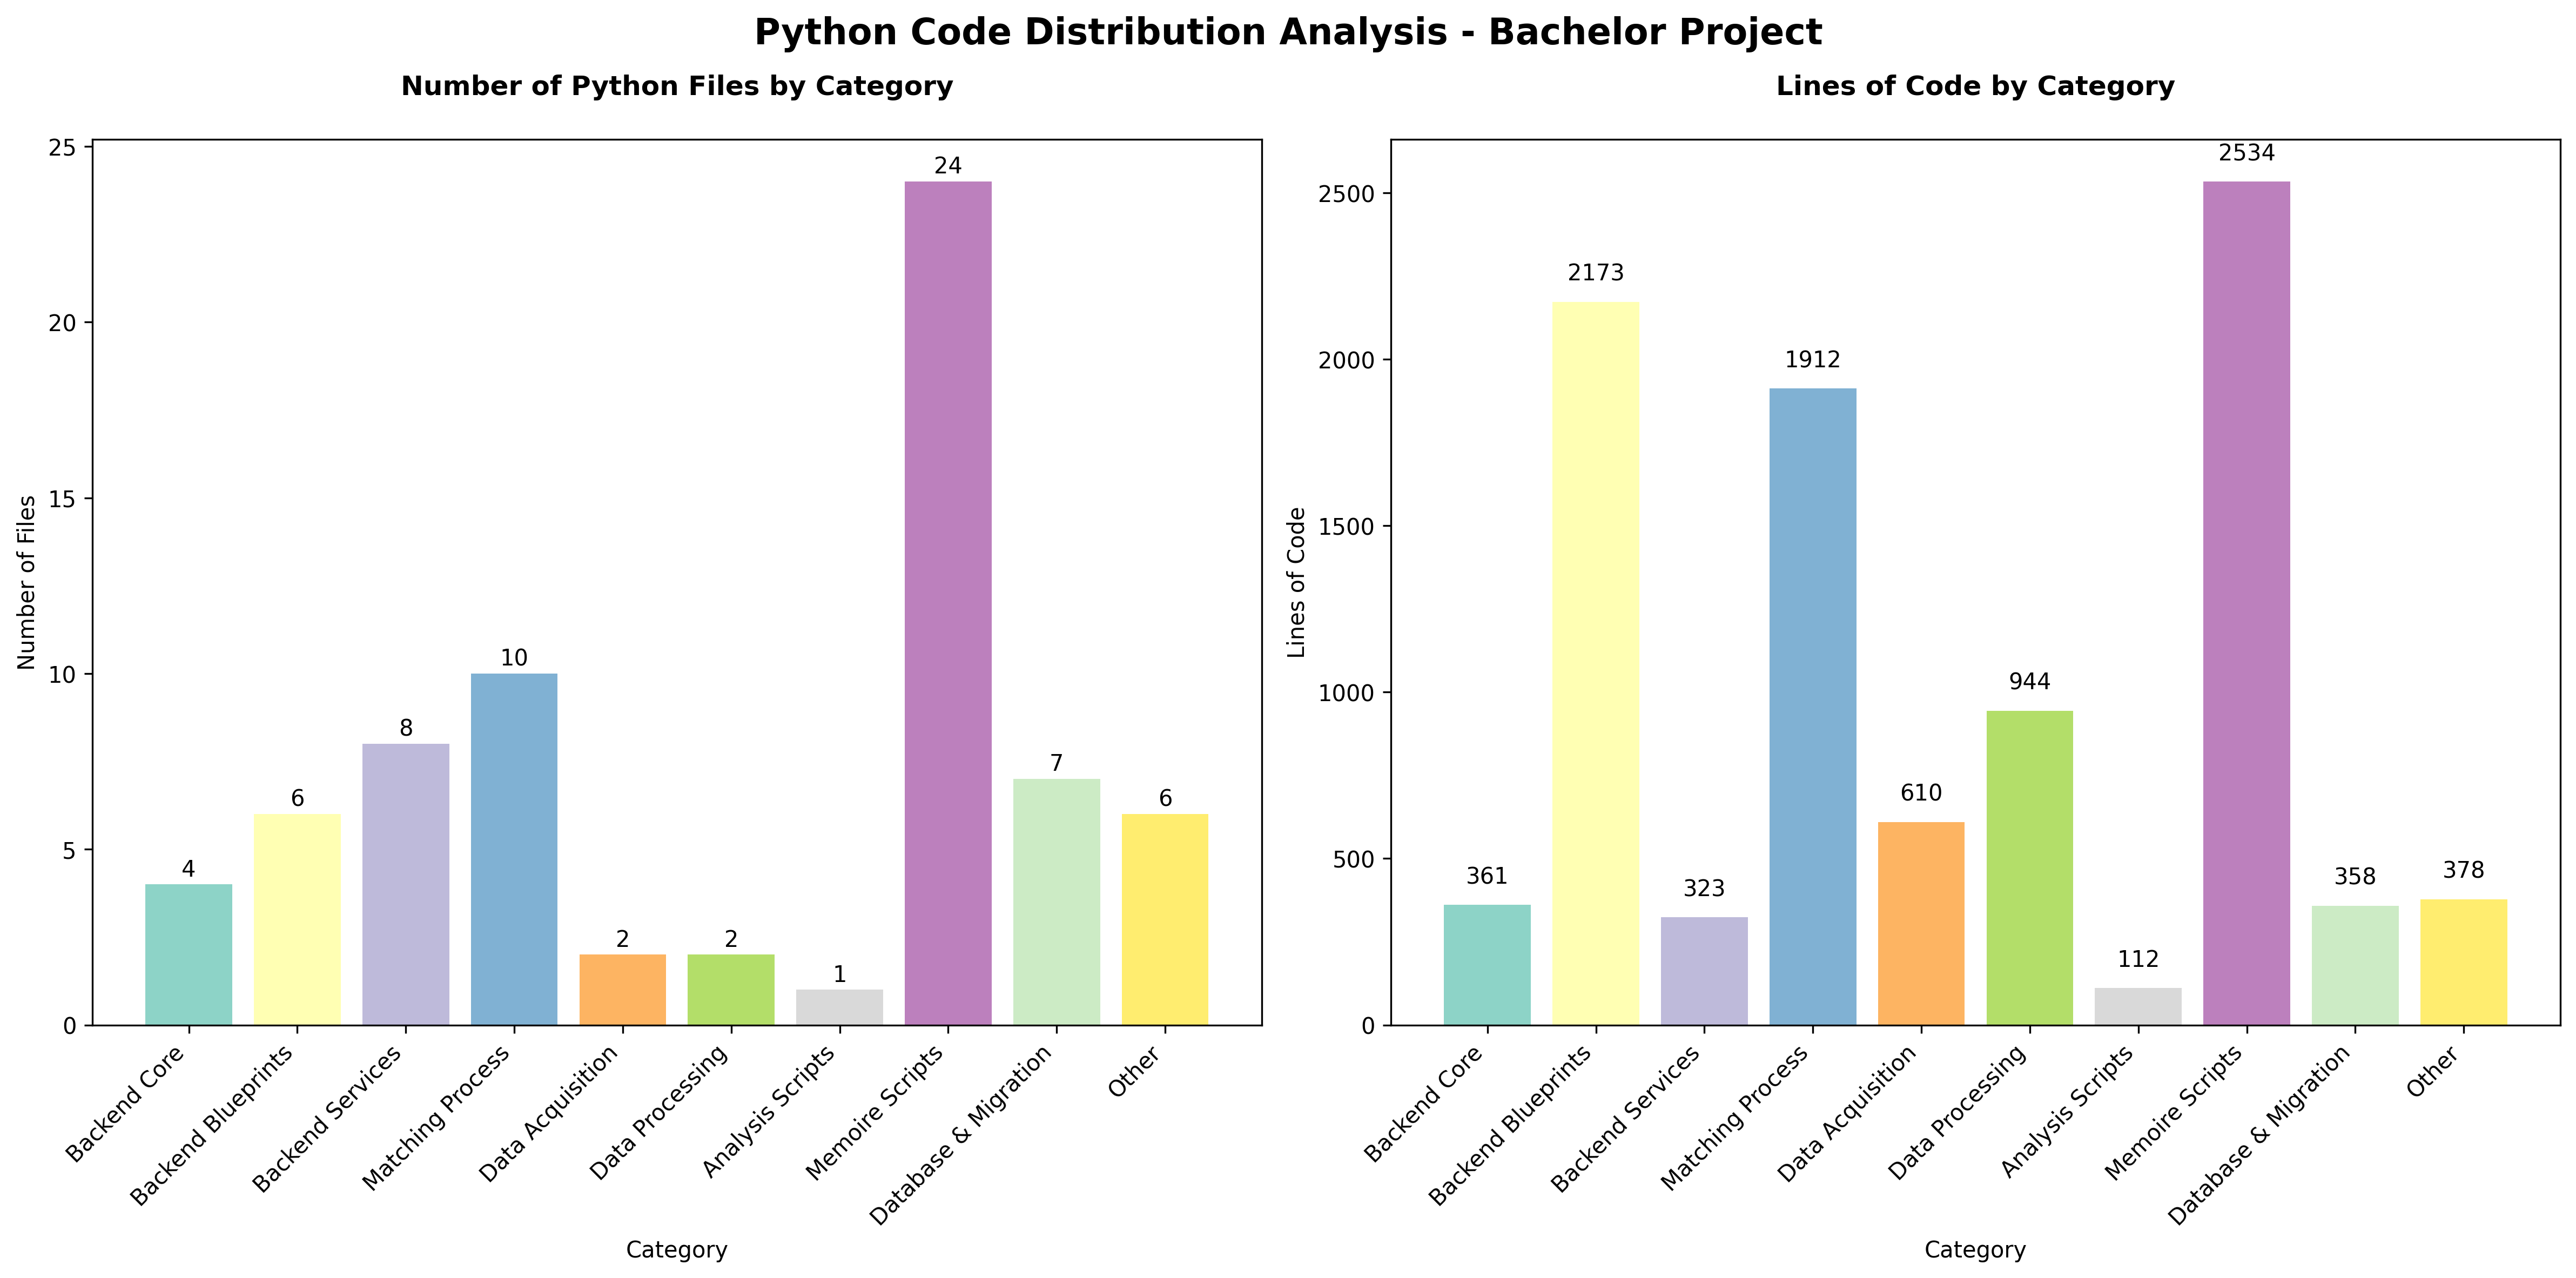
\includegraphics[width=\textwidth]{figures/conclusion/python_distribution_analysis.png}
\caption{Distribution du code Python : nombre de fichiers par catégorie (gauche) et lignes de code par catégorie (droite)}
\label{fig:python_distribution}
\end{figure}


\section*{Bilan personnel et réflexif}

Au-delà de ses objectifs techniques, ce projet a constitué une expérience d'apprentissage exceptionnellement riche et transversale. Sur le plan technique, il m'a permis d'acquérir et de consolider des compétences dans des domaines variés : du traitement des données à la conception d'algorithmes, en passant par le développement d'une application web complète, la sécurisation des API, la conception et l’implémentation d’un système d’authentification, ainsi que le déploiement par conteneurisation.
J’ai également acquis des compétences de domaine, en me familiarisant avec différents jeux de données du monde du transport public (GTFS, HRDF). J’ai beaucoup appris sur OpenStreetMap, des connaissances utiles pour de nombreux projets.

Le défi consistant à rendre des données brutes et hétérogènes non seulement intelligibles mais aussi exploitables via une interface utilisateur intuitive a été particulièrement stimulant.
La conception de l’interface utilisateur a été l’un des aspects les plus délicats : sélectionner et hiérarchiser l’information pertinente tout en préservant la simplicité d’usage.

Sur le plan de l'organisation et de la gestion de projet, ce travail m'a confronté à la nécessité d'une démarche structurée et à l'usage efficace d'outils comme Git et les IDE. La gestion des différentes facettes du projet – analyse de données, développement logiciel, rédaction technique – a exigé une planification rigoureuse et une capacité d'adaptation face aux difficultés rencontrées, que je considère comme autant d'opportunités d'apprentissage inhérentes au métier.

Ce qui m'a le plus passionné fut sans doute la dimension tangible de ce travail. Explorer les jeux de données, visualiser les réseaux de transport sur une carte et identifier des anomalies concrètes m'a offert une nouvelle perspective sur la géographie et l'infrastructure de la Suisse. La visite des bureaux des CFF à Berne fut également une expérience très enrichissante, qui a permis de contextualiser ce projet et de valider sa pertinence auprès d'experts du domaine.

\section*{Perspectives et améliorations futures}

Ce travail jette les bases d'un outil puissant, mais il ouvre également la voie à de nombreuses améliorations et extensions futures. Nous pouvons les regrouper en deux axes principaux.

Le premier axe concerne la \textbf{collaboration}. La prochaine étape à court terme est d'établir un canal de communication avec la communauté OpenStreetMap suisse afin de valider et d’itérer la solution et la méthode. Parallèlement, un processus de rétroaction devrait être mis en place pour signaler les incohérences avérées à l'équipe ATLAS. Pour pérenniser le projet, il serait également pertinent de le structurer en open-source, en définissant des lignes directrices pour les contributions externes.

Le deuxième axe porte sur les \textbf{améliorations techniques}. Les algorithmes d'appariement pourraient être affinés, par exemple par un modèle de scoring (éventuellement basé sur l'apprentissage automatique) qui attribuerait un score de confiance à chaque correspondance potentielle. L'application web pourrait bénéficier de fonctionnalités avancées, telles qu’une meilleure interface de résolution de problèmes pour les résoudre en masse ou encore des tableaux pour suivre l'évolution de la qualité des données.

\vspace{0.5em}
\section*{Conclusion}

\newline

Pas toujours fluide, parfois en correspondance serrée, mais au final ce projet est bien allé jusqu’au terminus.
